\documentclass[11pt,a4paper]{article}

\usepackage[margin=1in]{geometry}
\usepackage{amsmath}
\usepackage{booktabs}
\usepackage{tabularx}
\usepackage{hyperref}
\usepackage{tikz}
\usetikzlibrary{arrows.meta,positioning}
\usepackage{xcolor}
\usepackage{fancyhdr}

\hypersetup{colorlinks=true,linkcolor=black,urlcolor=blue}
\pagestyle{fancy}
\fancyhf{}
\fancyhead[L]{\small CSE 406 Design Proposal}
\fancyhead[R]{\small Project 20}
\fancyfoot[C]{\thepage}
\renewcommand{\headrulewidth}{0.4pt}

\begin{document}

\begin{center}
{\LARGE\bfseries Design Proposal}\\[0.35em]
{\large Project 20: Wi-Fi Password Cracking Attack}\\[0.5em]
\begin{tabular}{rl}
Student: & Mohammad Saifuzzaman \\
ID: & 2105088 \\
Section / Group: & B1 --- Group 3 \\
\end{tabular}
\end{center}

\vspace{0.4em}
\noindent\rule{\textwidth}{0.4pt}
\vspace{0.3em}

\noindent\textit{Updated per supervisor: multiple attacks on one setup; attacks run on
captured pcap files (public sample pcaps allowed).}

%----------------------------------------------------------------------
\section{Overview of the Project Idea}

\textbf{Setup (one):} Own offline tool that reads 802.11 pcaps, parses EAPOL,
and recovers WPA2-PSK passphrases. Same host, same code base, same workflow.

\textbf{Multiple attacks on that setup:}
\begin{enumerate}
  \item \textbf{Handshake MIC dictionary} --- verify candidates against 4-way
        handshake MIC (He \& Mitchell, 2004/2005).
  \item \textbf{PMKID dictionary} --- verify candidates against PMKID
        (CERT-EU SA2018-019, 2018).
  \item \textbf{Mask / limited brute} --- same verifiers, but candidates from a
        pattern (e.g.\ digits/short masks) instead of a wordlist.
\end{enumerate}

Input = \textbf{pcap} (public demo/sample captures from the Internet, and/or our
own lab capture). Cracking code is \textbf{ours} (Python/C; \texttt{hashlib}/\texttt{hmac}).
No aircrack-ng / Hashcat.

\textbf{Defense:} Strong PSK + \textbf{WPA3-SAE-only} (RFC~7664; Lancrenon \&
\v{S}krobot~2015). Avoid WPA2 transition mode (Dragonblood, 2020).

%----------------------------------------------------------------------
\section{Network Topology, Components and Timing Diagram}

\subsection{Topology (one setup)}
\begin{center}
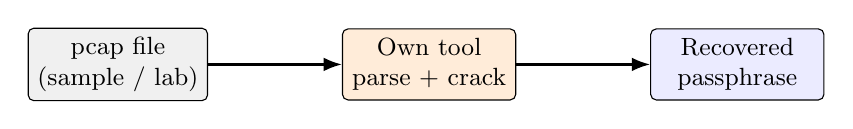
\begin{tikzpicture}[
  node distance=1.35cm and 1.7cm,
  box/.style={draw,rounded corners=2pt,align=center,minimum width=2.2cm,
              minimum height=0.9cm,font=\small},
  arr/.style={-{Latex},thick}
]
  \node[box,fill=gray!12] (pcap) {pcap file\\(sample / lab)};
  \node[box,fill=orange!15,right=of pcap] (tool) {Own tool\\parse + crack};
  \node[box,fill=blue!8,right=of tool] (out) {Recovered\\passphrase};
  \draw[arr] (pcap) -- (tool);
  \draw[arr] (tool) -- (out);
\end{tikzpicture}
\end{center}

\noindent Optional lab AP/STA only to \emph{produce} a pcap. Demo attacks run
\textbf{on pcaps}, not against live foreign networks.

\subsection{Components}
\begin{center}
\begin{tabularx}{\textwidth}{@{}l X@{}}
\toprule
\textbf{Part} & \textbf{Role} \\
\midrule
pcap input & Public sample WPA2 handshake/PMKID captures; optional own lab capture. \\
Own tool & One pipeline: parse $\rightarrow$ Attack~1 / 2 / 3 $\rightarrow$ result. \\
Wordlist / mask & Candidates for dictionary vs mask modes. \\
Defense notes & WPA3-SAE-only + strong passphrase checklist. \\
\bottomrule
\end{tabularx}
\end{center}

\subsection{Timing --- handshake (in pcap)}
\begin{center}
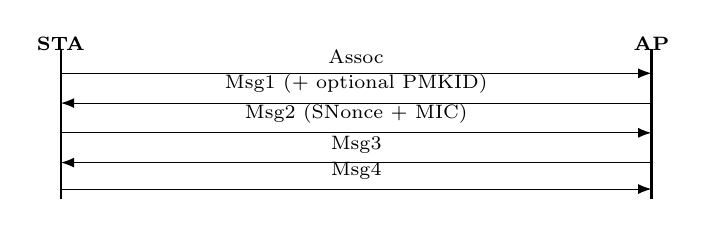
\begin{tikzpicture}[x=2.5cm,y=0.42cm,font=\scriptsize]
  \node at (0,0) {\textbf{STA}}; \node at (3,0) {\textbf{AP}};
  \draw[thick] (0,-0.15)--(0,-4.7); \draw[thick] (3,-0.15)--(3,-4.7);
  \draw[-{Latex}] (0,-0.9)--(3,-0.9) node[midway,above]{Assoc};
  \draw[-{Latex}] (3,-1.8)--(0,-1.8) node[midway,above]{Msg1 (+ optional PMKID)};
  \draw[-{Latex}] (0,-2.7)--(3,-2.7) node[midway,above]{Msg2 (SNonce + MIC)};
  \draw[-{Latex}] (3,-3.6)--(0,-3.6) node[midway,above]{Msg3};
  \draw[-{Latex}] (0,-4.4)--(3,-4.4) node[midway,above]{Msg4};
\end{tikzpicture}
\end{center}

\subsection{Timing --- attacks (offline on pcap)}
Load pcap $\rightarrow$ extract EAPOL fields $\rightarrow$ run Attack~1, then~2,
then~3 on the same capture (when fields exist) $\rightarrow$ report passphrase
or ``not found.''

%----------------------------------------------------------------------
\section{Packet and Frame Structure}

\begin{center}
\begin{tabularx}{\textwidth}{@{}l X@{}}
\toprule
\textbf{Layer} & \textbf{Fields} \\
\midrule
Radiotap / 802.11 & Enough to locate data/EAPOL frames; MACs / BSSID. \\
LLC/SNAP & EtherType \texttt{0x888E}. \\
EAPOL-Key & ANonce, SNonce, MIC, Key Data (PMKID / RSN IE). \\
\bottomrule
\end{tabularx}
\end{center}

\vspace{0.25em}
\noindent PMK = PBKDF2-HMAC-SHA1(passphrase, SSID, 4096, 32)\\
Attack~1: PTK from PMK + nonces + MACs; match MIC.\\
Attack~2: PMKID = HMAC-SHA1-128(PMK, ``PMK Name'' $\|$ MAC$_{AP}$ $\|$ MAC$_{STA}$).\\
Attack~3: same checks; different candidate generator (mask).

%----------------------------------------------------------------------
\section{Implementation Plan}

\begin{enumerate}
  \item Collect sample WPA2 pcaps (public demo captures) + small wordlist/mask.
  \item Build pcap reader + EAPOL parser (own code).
  \item Implement Attack~1 (MIC), Attack~2 (PMKID), Attack~3 (mask).
  \item Demo all three on the same setup/pcap set.
  \item Defense section: strong PSK + WPA3-SAE-only; Dragonblood caveat.
\end{enumerate}

\noindent\textbf{Modules:} \texttt{pcap/}, \texttt{parse/}, \texttt{crypto/},
\texttt{attack\_mic/}, \texttt{attack\_pmkid/}, \texttt{attack\_mask/},
\texttt{defend/}.

%----------------------------------------------------------------------
\section{Expected Outcome of a Successful Attack}

\begin{itemize}
  \item Attack~1 recovers passphrase from a handshake pcap when it is in the list.
  \item Attack~2 recovers passphrase from a PMKID-bearing pcap when present.
  \item Attack~3 recovers a short/pattern passphrase via mask within demo time.
  \item Wrong candidates fail; missing fields $\rightarrow$ that attack reports N/A.
  \item Defense contrast: WPA3-SAE is not crackable by these WPA2 offline methods.
\end{itemize}

%----------------------------------------------------------------------
\section{Defense Idea}

\begin{enumerate}
  \item Long, non-dictionary passphrase.
  \item Prefer \textbf{WPA3-SAE-only} (disable WPA2 transition).
  \item Optional helper: warn if capture/settings imply WPA2-PSK only.
\end{enumerate}

\noindent Dragonblood (2020): keep SAE implementations updated; avoid compatibility
mode that re-enables WPA2-style offline cracking paths.

\end{document}
